%%%%%%%%%%%%%%%%%%%%%%%%%%%%%%%%%%%%
%% PREAMBLE
%%%%%%%%%%%%%%%%%%%%%%%%%%%%%%%%%%%%

\documentclass[11pt]{article}

% packages needed for state diagrams
\usepackage{pgf}
\usepackage{tikz}
\usetikzlibrary{arrows,automata}

% package needed for parse trees
\usepackage{tikz-qtree}

% nice clickable URLs
\usepackage{url}

% page margins
\usepackage[margin=2.5cm]{geometry}
\setlength{\parindent}{0pt}

% math
\usepackage{amsmath,amssymb}

\begin{document}

%%%%%%%%%%%%%%%%%%%%%%%%%%%%%%%%%%%%
%% HEADING
%%%%%%%%%%%%%%%%%%%%%%%%%%%%%%%%%%%%

\rule{\textwidth}{1pt}
\begin{center}
  \textbf{Taaltheorie en Taalverwerking -- Homework Submission}
\end{center}
\rule{\textwidth}{0.5pt}\\

%%%%%%%%%%%%%%%%%%%%%%%%%%%%%%%%%%%%
%% ENTER DETAILS
%%%%%%%%%%%%%%%%%%%%%%%%%%%%%%%%%%%%

\textbf{Week:} 2

\textbf{Group:} 28

\textbf{Student names and IDs:} Bob Engel 12627143, Dion Streefkerk 15847195

\textbf{Date:} April 12, 2026

\rule{\textwidth}{1pt}

%%%%%%%%%%%%%%%%%%%%%%%%%%%%%%%%%%%%
%% YOUR ANSWERS
%%%%%%%%%%%%%%%%%%%%%%%%%%%%%%%%%%%%

\begin{enumerate}

%% ============================================================
%% EXERCISE 1
%% ============================================================
\item \textbf{Constituentenstructuur en parse trees.}

%% --- 1(a) ---
\begin{enumerate}
\item \textbf{``The paper on LLMs is in the reader.''}

\textbf{Aantal parse trees: 1}

Het subject-NP moet ``The paper on LLMs'' zijn, omdat de VP moet beginnen met een werkwoord (V = ``is'') en er geen woorden v\'o\'or ``is'' bij de VP kunnen horen. Er is slechts \'e\'en manier om dit NP op te bouwen (via Nom $\to$ Nom PP). Voor de VP ``is in the reader'' is de enige toepasbare regel VP $\to$ V PP (VP $\to$ V NP werkt niet omdat ``in'' geen NP kan beginnen; VP $\to$ V NP PP kan ``in the reader'' niet opsplitsen in NP + PP).

\bigskip
\begin{center}
\Tree[.S [.NP [.Det the ] [.Nom [.Nom [.N paper ] ] [.PP [.P on ] [.NP [.PN LLMs ] ] ] ] ] [.VP [.V is ] [.PP [.P in ] [.NP [.Det the ] [.Nom [.N reader ] ] ] ] ] ]
\end{center}

%% --- 1(b) ---
\item \textbf{``I returned a paper to the library.''}

\textbf{Aantal parse trees: 2}

NP $=$ ``I'' (Pro). De VP ``returned a paper to the library'' kan op twee manieren geparsed worden:

\begin{itemize}
\item \textbf{Tree 1} --- VP $\to$ V NP, waarbij NP $=$ ``a paper to the library''.
Hier geldt NP $\to$ Det Nom, en Nom $\to$ Nom PP hecht ``to the library'' aan als bepaling bij ``paper''. Semantisch onlogisch: het zou een paper beschrijven dat naar de bibliotheek gaat.

\item \textbf{Tree 2} --- VP $\to$ V NP PP, waarbij NP $=$ ``a paper'' en PP $=$ ``to the library''.
Hier is de PP een argument van het ditransitieve werkwoord ``returned''. Dit komt overeen met de bedoelde betekenis.
\end{itemize}

\textbf{Correcte parse tree (Tree 2):}

\bigskip
\begin{center}
\Tree[.S [.NP [.Pro I ] ] [.VP [.V returned ] [.NP [.Det a ] [.Nom [.N paper ] ] ] [.PP [.P to ] [.NP [.Det the ] [.Nom [.N library ] ] ] ] ] ]
\end{center}

%% --- 1(c) ---
\item \textbf{``I read an essay about ethics.''}

\textbf{Aantal parse trees: 2}

NP $=$ ``I'' (Pro). De VP ``read an essay about ethics'' kan op twee manieren geparsed worden:

\begin{itemize}
\item \textbf{Tree 1} --- VP $\to$ V NP, waarbij NP $=$ ``an essay about ethics''.
Hier hecht Nom $\to$ Nom PP de PP ``about ethics'' aan ``essay''. Semantisch correct: een essay waarvan het onderwerp ethiek is.

\item \textbf{Tree 2} --- VP $\to$ V NP PP, waarbij NP $=$ ``an essay'' en PP $=$ ``about ethics''.
Hier modificeert de PP de VP in plaats van het zelfstandig naamwoord. Semantisch minder natuurlijk.
\end{itemize}

\textbf{Correcte parse tree (Tree 1):}

\bigskip
\begin{center}
\Tree[.S [.NP [.Pro I ] ] [.VP [.V read ] [.NP [.Det an ] [.Nom [.Nom [.N essay ] ] [.PP [.P about ] [.NP [.PN ethics ] ] ] ] ] ] ]
\end{center}

%% --- 1(d) ---
\item \textbf{Waarom kan de grammatica oneindig veel zinnen genereren?}

De grammatica kan oneindig veel zinnen genereren vanwege \textbf{indirecte recursie} via drie regels:

\begin{enumerate}
\item[1.] Nom $\to$ Nom PP
\item[2.] PP $\to$ P NP
\item[3.] NP $\to$ Det Nom
\end{enumerate}

Deze regels vormen een cyclus: een Nom kan expanderen naar Nom PP, die een NP bevat (via PP $\to$ P NP), die op zijn beurt een nieuwe Nom bevat (via NP $\to$ Det Nom). Deze nieuwe Nom kan opnieuw expanderen via Nom $\to$ Nom PP, enzovoort tot in het oneindige.

Voorbeeld: ``the paper on LLMs in the reader on the essay about the library in the paper \ldots''

Elke expansie voegt een nieuwe PP toe, en dit proces kan onbegrensd herhaald worden, wat een oneindig aantal verschillende zinnen oplevert.

%% --- 1(e) ---
\item \textbf{Parsen van ``Which paper do you like?''}

De volgende regels moeten worden toegevoegd:

\textbf{Nieuwe lexicale regels:}
\begin{itemize}
\item Det $\to$ which
\item Aux $\to$ do \quad (nieuwe lexicale categorie voor hulpwerkwoorden)
\end{itemize}

\textbf{Nieuwe phrase structure regels:}
\begin{itemize}
\item S $\to$ NP Aux NP VP \quad (wh-vraagstructuur; 4-weg vertakking)
\item VP $\to$ V \quad (kaal werkwoord zonder object, omdat het object naar voren is verplaatst)
\end{itemize}

\textbf{Parse tree:}

\bigskip
\begin{center}
\Tree[.S [.NP [.Det which ] [.Nom [.N paper ] ] ] [.Aux do ] [.NP [.Pro you ] ] [.VP [.V like ] ] ]
\end{center}

\end{enumerate}

%% ============================================================
%% EXERCISE 2
%% ============================================================
\item \textbf{Formele taal} $L = \{x \mid x \text{ bevat een even aantal 0'en gevolgd door een even aantal 1'en}\}$

De taal bestaat uit strings van de vorm $(00)^n(11)^m$ met $n, m \geq 0$.

%% --- 2(a) ---
\begin{enumerate}
\item \textbf{Reguliere expressie:}

$$(00)^*(11)^*$$

%% --- 2(b) ---
\item \textbf{FSA:}

\begin{center}
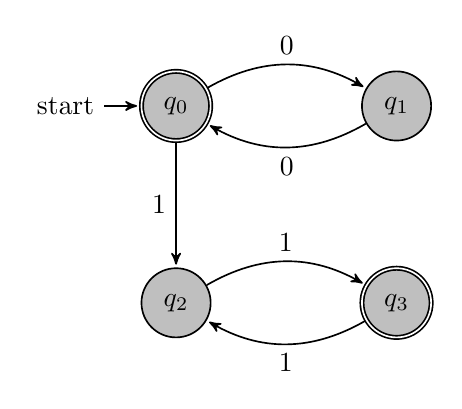
\begin{tikzpicture}[->,>=stealth',shorten >=1pt,auto,node distance=2.8cm,semithick]
  \tikzstyle{every state}=[fill=lightgray,draw=black,text=black]
\node[initial,state,accepting] (q0) {$q_0$};
\node[state] (q1) [right of=q0] {$q_1$};
\node[state] (q2) [below of=q0, node distance=2.5cm] {$q_2$};
\node[state,accepting] (q3) [right of=q2] {$q_3$};
\path
(q0) edge [bend left] node {0} (q1)
(q1) edge [bend left] node {0} (q0)
(q0) edge node[left] {1} (q2)
(q2) edge [bend left] node {1} (q3)
(q3) edge [bend left] node {1} (q2);
\end{tikzpicture}
\end{center}

Toestanden:
\begin{itemize}
\item $q_0$: starttoestand (accepterend). Even aantal 0'en gelezen, nog geen 1'en.
\item $q_1$: oneven aantal 0'en gelezen.
\item $q_2$: even aantal 0'en klaar, oneven aantal 1'en gelezen.
\item $q_3$: accepterend. Even aantal 0'en klaar, even aantal 1'en gelezen ($\geq 2$).
\end{itemize}

Opmerking: niet-getoonde overgangen leiden naar een impliciete dode toestand (bijv.\ een~1 lezen in $q_1$, of een~0 lezen in $q_2$ of~$q_3$).

%% --- 2(c) ---
\item \textbf{Right-linear grammatica:}

$\Sigma = \{0, 1\}$, \quad $N = \{q_0, q_1, q_2, q_3\}$, \quad $S = q_0$

Regels $R$:
\begin{align*}
q_0 &\to 0\, q_1 \\
q_0 &\to 1\, q_2 \\
q_0 &\to \varepsilon \\
q_1 &\to 0\, q_0 \\
q_2 &\to 1\, q_3 \\
q_3 &\to 1\, q_2 \\
q_3 &\to \varepsilon
\end{align*}

Deze grammatica is direct afgeleid van de FSA: elke transitie $(X, a) \to Y$ wordt een regel $X \to a\,Y$, en elke accepterende toestand $X$ krijgt een regel $X \to \varepsilon$.

%% --- 2(d) ---
\item \textbf{Pumping Lemma: conditie en voorbeeld.}

\textbf{Conditie:} Het Pumping Lemma stelt dat als $L$ een oneindige reguliere taal is, er dan een string $xyz \in L$ bestaat met $y \neq \varepsilon$ zodanig dat $xy^nz \in L$ voor alle $n \geq 0$.

\textbf{Voorbeeld:} Neem de string $0011 \in L$. Kies $x = \varepsilon$, $y = 00$, $z = 11$.

Dan geldt $xy^nz = (00)^n\,11$ voor alle $n \geq 0$:
\begin{itemize}
\item $n = 0$: $11$ --- 0 nullen (even), 2 enen (even) $\Rightarrow \in L$ \checkmark
\item $n = 1$: $0011$ --- 2 nullen (even), 2 enen (even) $\Rightarrow \in L$ \checkmark
\item $n = 2$: $000011$ --- 4 nullen (even), 2 enen (even) $\Rightarrow \in L$ \checkmark
\item Algemeen: $2n$ nullen (altijd even) gevolgd door 2 enen (even) $\Rightarrow \in L$ \checkmark
\end{itemize}

Aangezien er een decompositie $xyz$ bestaat met $y \neq \varepsilon$ zodanig dat $xy^nz \in L$ voor alle $n \geq 0$, voldoet de taal $L$ aan de pumping-conditie. Dit is consistent met het feit dat $L$ regulier is.

\end{enumerate}

%% ============================================================
%% EXERCISE 3
%% ============================================================
\item \textbf{Taal} $L = \{a^{2n}\, b^3\, a^{2n} \mid n \geq 0\}$

Strings in $L$: $bbb$, $aabbbaa$, $aaaabbbaaaa$, $\ldots$

%% --- 3(a) ---
\begin{enumerate}
\item \textbf{Is $L$ regulier?}

\textbf{Nee, $L$ is niet regulier.}

\textbf{Bewijs met het Pumping Lemma:}

Neem aan dat $L$ regulier is. Dan geldt volgens het Pumping Lemma: er bestaat een string $xyz \in L$ met $y \neq \varepsilon$ zodanig dat $xy^mz \in L$ voor alle $m \geq 0$.

Beschouw een willekeurige string $s = a^{2n}\,bbb\,a^{2n} \in L$. Schrijf $s = xyz$ met $y \neq \varepsilon$. We onderzoeken alle mogelijke posities van $y$.

\textit{Geval $n = 0$:} $s = bbb$. Hier kan $y$ alleen uit $b$'s bestaan, wat valt onder Geval~2 hieronder.

\textit{Geval $n \geq 1$:} We krijgen de volgende mogelijkheden:

\textbf{Geval 1:} $y$ bestaat alleen uit $a$'s uit de eerste groep ($y = a^i$, $i > 0$).

Pomp met $m = 0$: $xy^0z = a^{2n-i}\,bbb\,a^{2n}$. Omdat $i > 0$ verschilt het aantal $a$'s v\'o\'or $bbb$ ($2n - i$) van het aantal erna ($2n$). Niet in $L$. $\Rightarrow\!\Leftarrow$

\textbf{Geval 2:} $y$ bestaat alleen uit $b$'s ($y = b^i$, $1 \leq i \leq 3$).

Pomp met $m = 0$: $xy^0z$ bevat $3 - i < 3$ keer $b$ in het midden. Niet in $L$. $\Rightarrow\!\Leftarrow$

\textbf{Geval 3:} $y$ overlapt de grens tussen de eerste $a$'s en $b$'s ($y = a^i b^j$, $i > 0$, $j > 0$).

Pomp met $m = 2$: $xy^2z$ bevat de deelstring $b^j a^i b^j$, d.w.z.\ er verschijnen $a$'s tussen $b$'s. De resulterende string past niet in het patroon $a^*\,b^3\,a^*$. Niet in $L$. $\Rightarrow\!\Leftarrow$

\textbf{Geval 4:} $y$ bestaat alleen uit $a$'s uit de tweede groep ($y = a^i$, $i > 0$).

Pomp met $m = 0$: $xy^0z = a^{2n}\,bbb\,a^{2n-i}$. De twee groepen $a$'s zijn ongelijk. Niet in $L$. $\Rightarrow\!\Leftarrow$

\textbf{Geval 5:} $y$ overlapt de grens tussen $b$'s en de tweede $a$'s ($y = b^i a^j$, $i > 0$, $j > 0$).

Pomp met $m = 2$: $xy^2z$ bevat $a$'s die afgewisseld worden met $b$'s. Niet in $L$. $\Rightarrow\!\Leftarrow$

In alle gevallen leidt pompen tot een string buiten $L$. Dit is een tegenspraak met de aanname dat $L$ regulier is.

$\therefore$ $L$ is niet regulier. \hfill $\square$

%% --- 3(b) ---
\item \textbf{Is $L$ context-vrij?}

\textbf{Ja, $L$ is context-vrij.} De volgende context-vrije grammatica genereert $L$:

$\Sigma = \{a, b\}$, \quad $N = \{S\}$, \quad startsymbool: $S$

Regels $R$:
\begin{align*}
S &\to a\,a\,S\,a\,a \\
S &\to b\,b\,b
\end{align*}

\textbf{Verificatie:}
\begin{itemize}
\item $n = 0$: $S \Rightarrow bbb$ \checkmark
\item $n = 1$: $S \Rightarrow aaSaa \Rightarrow aabbbaa$ \checkmark
\item $n = 2$: $S \Rightarrow aaSaa \Rightarrow aaaaSaaaa \Rightarrow aaaabbbaaaa$ \checkmark
\item Algemeen: $n$ keer $S \to aaSaa$ toepassen en daarna $S \to bbb$ levert $a^{2n}\,bbb\,a^{2n}$ op. \checkmark
\end{itemize}

De regel $S \to aaSaa$ voegt steeds twee $a$'s aan beide kanten toe, waardoor de aantallen gelijk en even blijven. Dit is een context-vrije grammatica omdat elke regel precies \'e\'en niet-terminaal symbool aan de linkerkant heeft.

\end{enumerate}

\end{enumerate}

%%%%%%%%%%%%%%%%%%%%%%%%%%%%%%%%%%%%
%% END
%%%%%%%%%%%%%%%%%%%%%%%%%%%%%%%%%%%%

\end{document}
